%%%%%%%%%%%%%%%%%%%%%%%%%%%%%%%%%%%%%%%%%
% Journal Article
% LaTeX Template
% Version 1.4 (15/5/16)
%
% This template has been downloaded from:
% http://www.LaTeXTemplates.com
%
% Original author:
% Frits Wenneker (http://www.howtotex.com) with extensive modifications by
% Vel (vel@LaTeXTemplates.com)
%
% License:
% CC BY-NC-SA 3.0 (http://creativecommons.org/licenses/by-nc-sa/3.0/)
%
%%%%%%%%%%%%%%%%%%%%%%%%%%%%%%%%%%%%%%%%%

%----------------------------------------------------------------------------------------

%	PACKAGES AND OTHER DOCUMENT CONFIGURATIONS
%----------------------------------------------------------------------------------------
\documentclass[twoside,twocolumn]{article}

\usepackage[sc]{mathpazo} % Use the Palatino font
\usepackage[T1]{fontenc} % Use 8-bit encoding that has 256 glyphs
%\linespread{1.05} % Line spacing - Palatino needs more space between lines
\usepackage{microtype} % Slightly tweak font spacing for aesthetics

\usepackage[english]{babel} % Language hyphenation and typographical rules

\usepackage[hmarginratio=1:1,top=32mm,columnsep=20pt]{geometry} % Document margins
\usepackage[hang, small,labelfont=bf,up]{caption} % Custom captions under/above floats in tables or figures
\usepackage{booktabs} % Horizontal rules in tables

\usepackage{lettrine} % The lettrine is the first enlarged letter at the beginning of the text

\usepackage{enumitem} % Customized lists
\setlist[itemize]{noitemsep} % Make itemize lists more compact

\usepackage{abstract} % Allows abstract customization
\renewcommand{\abstractnamefont}{\normalfont\bfseries} % Set the "Abstract" text to bold
\renewcommand{\abstracttextfont}{\normalfont\small\itshape} % Set the abstract itself to small italic text

\usepackage{titlesec} % Allows customization of titles
\renewcommand\thesection{\Roman{section}} % Roman numerals for the sections
\renewcommand\thesubsection{\roman{subsection}} % roman numerals for subsections
\titleformat{\section}[block]{\large\scshape\centering}{\thesection.}{1em}{} % Change the look of the section titles
\titleformat{\subsection}[block]{\large}{\thesubsection.}{1em}{} % Change the look of the section titles

\usepackage{fancyhdr} % Headers and footers
%\pagestyle{fancy} % All pages have headers and footers
%\fancyhead{} % Blank out the default header
%\fancyfoot{} % Blank out the default footer
%\fancyhead[C]{Running title $\bullet$ May 2016 $\bullet$ Vol. XXI, No. 1} % Custom header text
%\fancyfoot[RO,LE]{\thepage} % Custom footer text

\usepackage{titling} % Customizing the title section

\usepackage{hyperref} % For hyperlinks in the PDF

\usepackage{graphicx}
\usepackage[tbtags]{amsmath}

%----------------------------------------------------------------------------------------
%	TITLE SECTION
%----------------------------------------------------------------------------------------

\setlength{\droptitle}{-4\baselineskip} % Move the title up

\pretitle{\begin{center}\Huge\bfseries} % Article title formatting
\posttitle{\end{center}} % Article title closing formatting
\title{Wireless/Bluetooth Communication} % Article title
\author{%
\textsc{Tian Ye} \\%\thanks{A thank you or further information} \\[1ex] % Your name
\normalsize 704-931-660 \\ % Your institution
\and % Uncomment if 2 authors are required, duplicate these 4 lines if more
\textsc{Aaron Philips} \\
\normalsize Lab Partner \\
\and
\textsc{Ryan Tong} \\
\normalsize Lab Partner \\
\and
\textsc{Kevin Zhang} \\%\thanks{Corresponding author} \\[1ex] % Second author's name
%\normalsize \href{mailto:jane@smith.com}{jane@smith.com} % Second author's email address
\normalsize Lab Partner \\
}
\date{Lab Section 1B} % Leave empty to omit a date
\renewcommand{\maketitlehookd}{%
\begin{abstract}
\noindent The two labs studied, Lab 1 and Lab 2, were designed to explore the concepts of data communication in wireless channels; namely, IEEE 802.11n wireless LAN and Bluetooth connections. We tested the relationship between distance and overall throughput and the effect of noise on wireless communication. Lab 1 focused on the effects of distance and microwave noise on TCP and UDP data channels, whilst Lab 2 focused on measuring data throughput of DH1, DH3, and DH5 packet types with the different factors in this lab being distance, connection interference via increasing the number of slave nodes, and data interference caused by Bluetooth and IEEE 802.11 devices.
\end{abstract}
}

%----------------------------------------------------------------------------------------

\begin{document}

% Print the title
\maketitle

%----------------------------------------------------------------------------------------
%	ARTICLE CONTENTS
%----------------------------------------------------------------------------------------

\section{Introduction: Wireless 802.11}

WiFi communication relies on channels known as 802.11 wireless, with differing subscripts depending version; the one used in the labs was 802.11b. Base communication has two major paradigms; the more popular being communication through a router or modem serving as a base station that broadcasts a wireless signal. In the event there is no base station, an ad-hoc network is used instead in which an access point is configured on one device that is connected to by all the other devices. 

\hfill

\noindent To prevent interference, wireless protocols rely on CSMA/CA (Carrier Sense Multiple Access/Collision Avoidance) which regulate flow on a given channel based on activity and also sense transmission from multiple carriers to regulate access protocol. Wireless LAN also utilizes DCF (Distributed Coordination Function), breaking up data into smaller packets to facilitate recovery of packets and distribution between multiple channels. The transport layer transfers data in two major ways:

\hfill

\noindent UDP is a connectionless protocol that does not require a handshake to establish packet transfer, and is characterized by extremely high throughput relative to other protocols and sends data as datagram packets. However, due to the lack of a handshake, there is no error detection of possibility of recovery: packets have the potential to be lost without warning or indication.

\hfill

\noindent TCP relies on an established connection that has a transmitter and a receiver, thus permitting two-way acknowledgments via the usage of CSMA/CA. Hence, it has error recovery, collision avoidance, and congestion control for the cost of lower throughput and expense. It is nonetheless far more prevalent as guarantee of package delivery is commonly a must.

%------------------------------------------------

\section{Introduction: Bluetooth}

While WLAN and Bluetooth both transmit over 2.4 Ghz, Bluetooth relies on Adaptive Frequency Hopping Spreading Spectrum (FHSS) rather than CSMA/CA. FHSS uses 79 frequency channels that utilize probability to prevent more than a number of Bluetooth channels be established at any given point of time. Further, fast hops between frequency channels are utilized to connect multiple devices. Consequently, Bluetooth has a much shorter range.

\hfill

\noindent Bluetooth uses an ad-hoc architecture where there is a master node and multiple slaves, where there can be up to 7 slaves per master. In order to avoid external interference, ACL and SCO links are used for packet-switching and real-time data, respectively; both do not require retransmission.

%------------------------------------------------

\section{Lab 1: Wireless 802.11b}

The various data collected from the lab is listed below:

\hfill

\begin{table}[!htbp]
\caption{Signal Strength vs Distance}
\centering
\scalebox{0.7}{
\begin{tabular}{cc}
\cmidrule{1-2}
Distance from Access Point (ft) & Signal Strength (dBm) \\
\midrule
30 & -34 \\
60 & -58 \\
90 & -60 \\
\bottomrule
\end{tabular}}
\end{table}

\begin{table}[!htbp]
\caption{Signal to Noise Ratio vs Distance}
\centering
\scalebox{0.7}{
\begin{tabular}{cc}
\cmidrule{1-2}
Distance from Access Point (ft) & Signal to Noise Ratio (dB) \\
\midrule
30 & 49 \\
60 & 24 \\
90 & 17 \\
\bottomrule
\end{tabular}}
\end{table}

\begin{table}[!htbp]
\caption{Signal to Noise Ratio vs TCP Throughput}
\centering
\scalebox{0.7}{
\begin{tabular}{cc}
\cmidrule{1-2}
Signal to Noise Ratio (dB) & TCP Data Throughput (Kbps) \\
\midrule
17 & 222 \\
24 & 518 \\
49 & 12200 \\
\bottomrule
\end{tabular}}
\end{table}

\begin{table}[!htbp]
\caption{Signal to Noise Ratio vs UDP Throughput}
\centering
\scalebox{0.7}{
\begin{tabular}{cc}
\cmidrule{1-2}
Signal to Noise Ratio (dB) & UDP Data Throughput (Kbps) \\
\midrule
17 & 318 \\
24 & 3590 \\
49 & 10200 \\
\bottomrule
\end{tabular}}
\end{table}

\begin{table}[!htbp]
\caption{UDP and TCP Throughput vs Microwave Settings}
\centering
\scalebox{0.7}{
\begin{tabular}{ccc}
\cmidrule{1-3}
 UDP Data (Mbps) & TCP Data (Mbps) & Microwave Setting\\
\midrule
0 & 18.3 & 10.3 \\
1 & 15 & 8.73 \\
2 & 16 & 9.43 \\
3 & 14.4 & 7.2 \\
4 & 10.3 & 6.48 \\
5 & 5.4 & 5.55 \\
\bottomrule
\end{tabular}}
\end{table}

\newpage

\noindent This lab sought to describe the variation of signal strength of UDP and TCP transactions as distance changed, as well as the effect of external interference on the connection. This was accomplished via varying the distance of a node laptop from a central server laptop and via microwave interference.  

\begin{figure}[htbp]
    \centering
    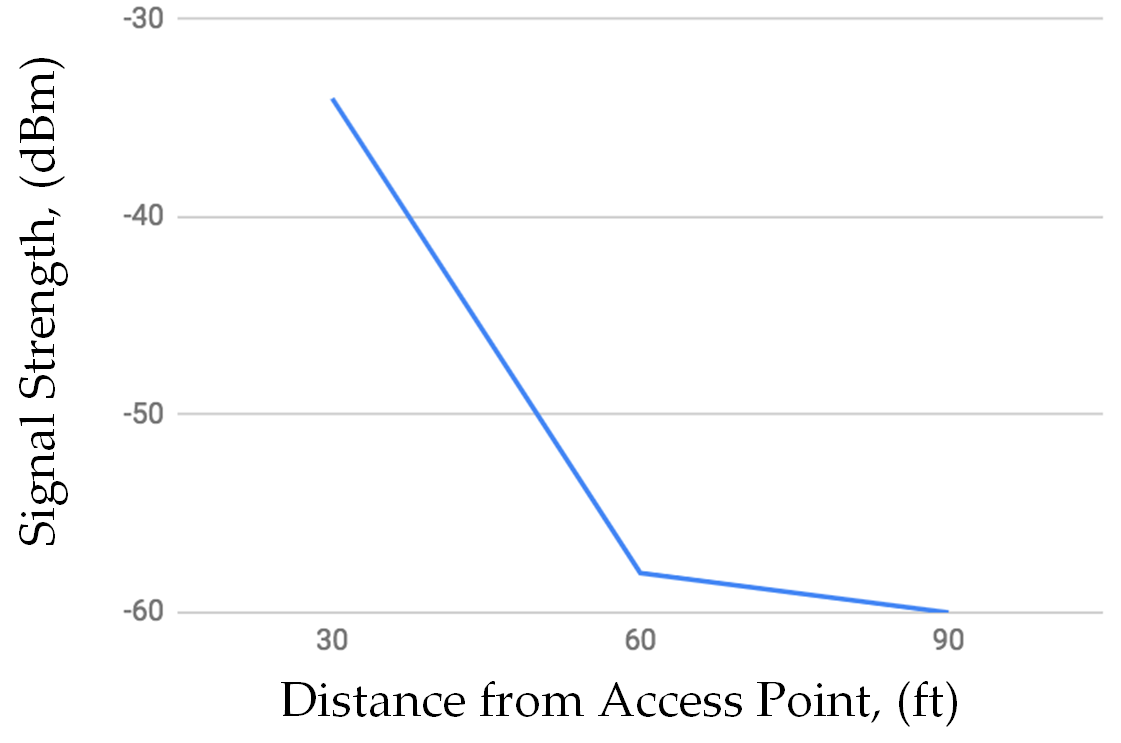
\includegraphics[width=2.9in]{StrDst.png}
    \caption{\textit{Signal Strength vs Distance from Access Point.} Note the exhibited inverse relation with distance.}
    \centering
    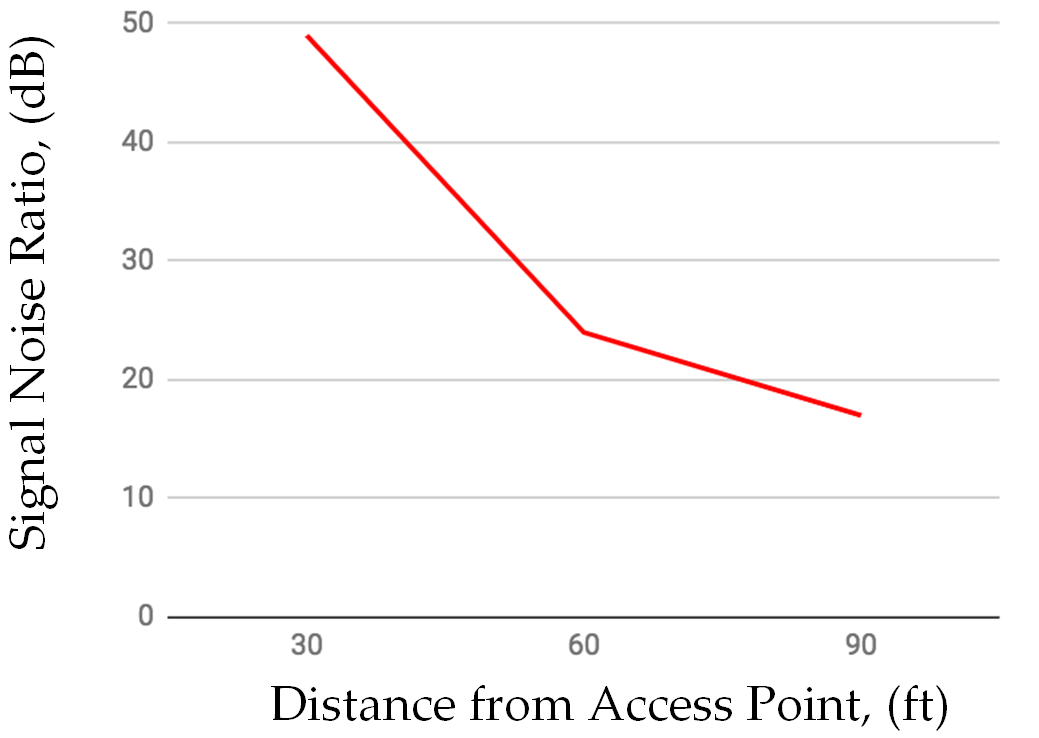
\includegraphics[width=2.9in]{SNR.png}
    \caption{\textit{Signal to Noise Ratio vs Distance from Access Point.} Once again, note the exhibited inverse relation with distance.}
\end{figure}

\noindent From Figure 1 and Figure 2, it can be theorized that noise levels increase with distance as a greater distance introduces a greater likelihood of disruption from external signals. This in turn causes signal strength to decrease as well: the signal is dispersed and corrupted with noise.

\newpage

\begin{figure}[htbp]
    \centering
    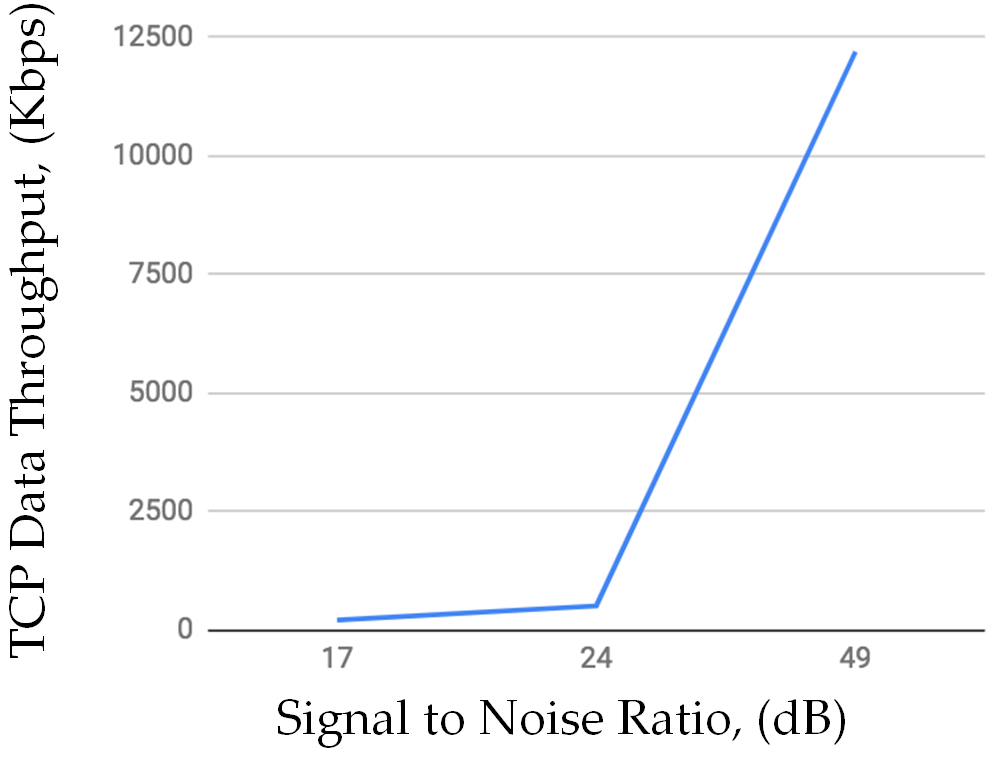
\includegraphics[width=2.9in]{TCP.png}
    \caption{\textit{TCP Data Throughput vs Signal to Noise Ratio.} Note the direct relationship between SNR and throughput.}
    \centering
    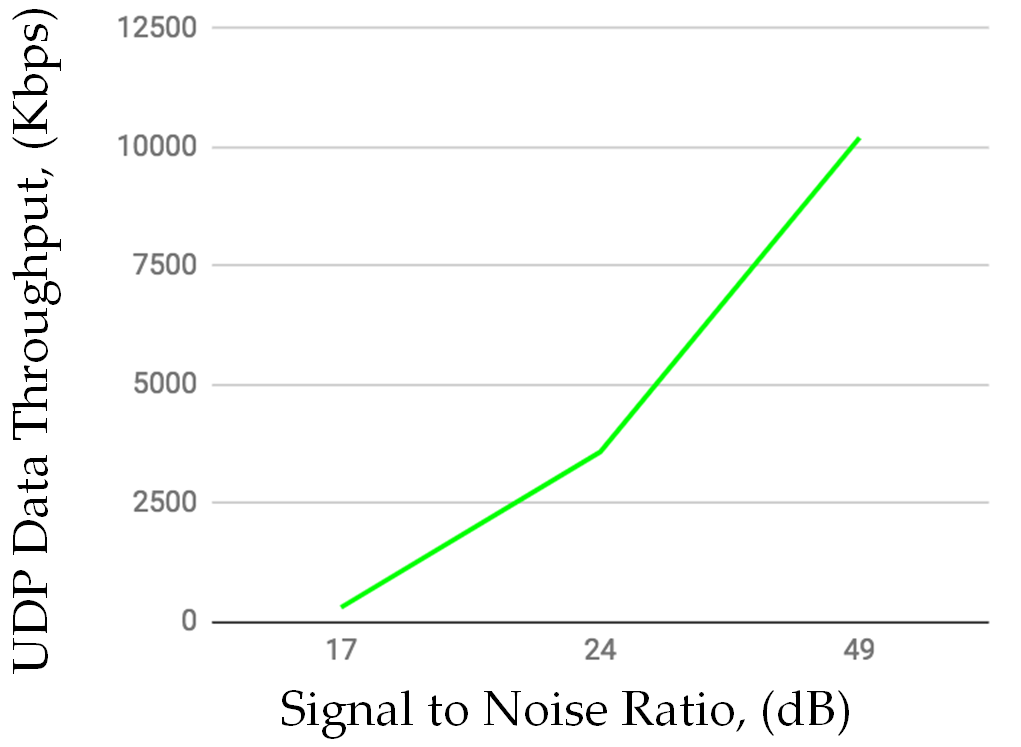
\includegraphics[width=2.9in]{UDP.png}
    \caption{\textit{UDP Data Throughput vs Signal to Noise Ratio.} Note the direct relationship between SNR and throughput.}
    \centering
    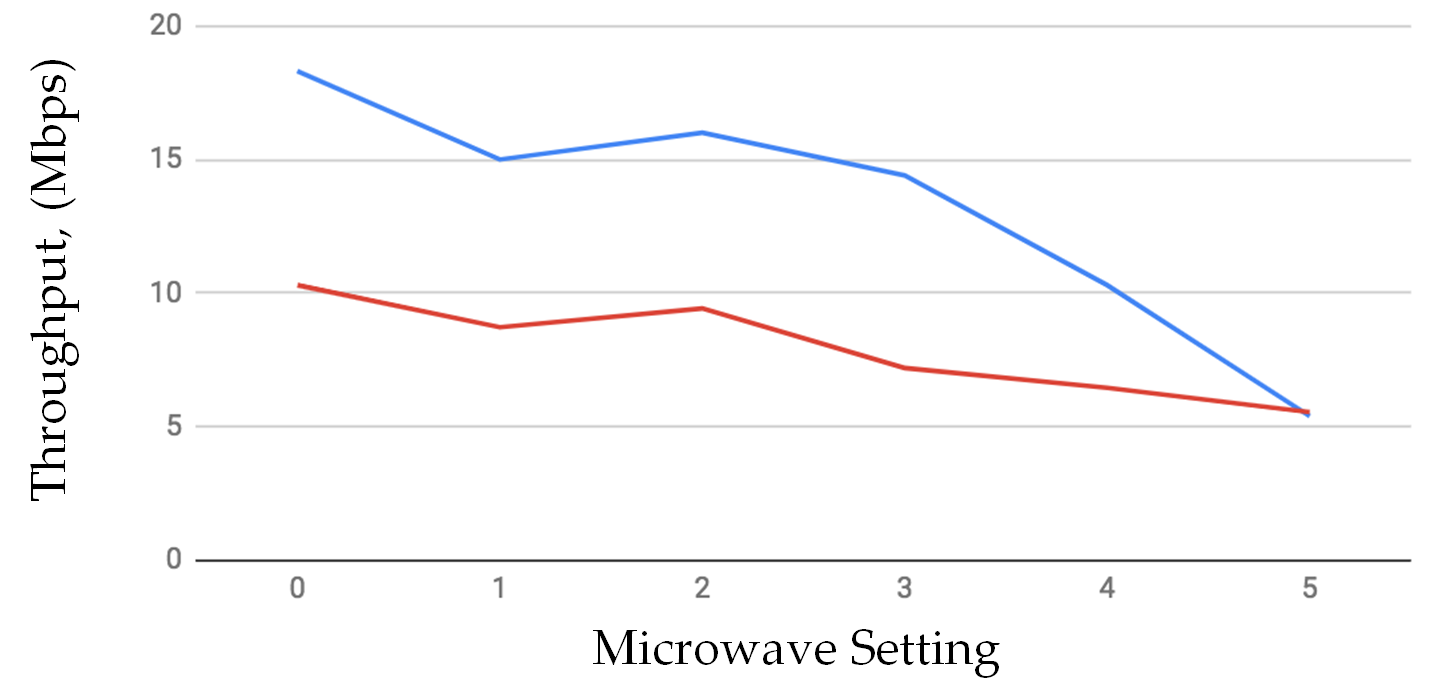
\includegraphics[width=2.9in]{Microwave.png}
    \caption{\textit{Throughput vs Microwave Settings.} The blue line corresponds to UDP whilst the red line corresponds to TCP. Note the data generally follows an inverse relation.}
\end{figure}
\noindent From Figure 2 and Figure 3, when comparing the signal strength of UDP and TCP to the signal to noise ratio, it can be seen that a higher ratio yields higher throughput, as lower noise results in a far more stable transfer of data.

\hfill 

\noindent In Figure 5, there exists a general trend in which as microwave level is increased, the throughput of both UDP and TCP data decreases. The noise can be attributed to extraneous sources, such as other experiments or other connections within the Boelter WLAN itself.

%------------------------------------------------

\section{Lab 2: Bluetooth}

The various data collected from the lab is listed below:

\hfill

\begin{table}[!htbp]
\caption{Bluetooth Throughput vs Distance}
\centering
\scalebox{0.7}{
\begin{tabular}{cccc}
\cmidrule{1-4}
Distance (m) & DH1 (Kbps) & DH3 (Kbps) & DH5 (Kbps) \\
\midrule
10 & 55.95 & 200.12 & 250.2 \\
15 & 48.2 & 100.03 & 177.46 \\
30 & 27.3 & 80.6 & 120.6  \\
\bottomrule
\end{tabular}}
\end{table}

\begin{table}[!htbp]
\caption{Bluetooth Throughput vs Number of Slaves}
\centering
\scalebox{0.7}{
\begin{tabular}{cccc}
\cmidrule{1-4}
No. of Slaves & DH1 (Kbps) & DH3 (Kbps) & DH5 (Kbps) \\
\midrule
1 &  56 & 197 & 263 \\
2 &  60 & 120 & 225 \\
3 &  30 & 90 & 150 \\
\bottomrule
\end{tabular}}
\end{table}

\begin{table}[!htbp]
\caption{Data Rate by Crossing Team}
\centering
\scalebox{0.7}{
\begin{tabular}{cc}
\cmidrule{1-2}
Crossing Teams & Data Throughput Per Connection (Kbps) \\
\midrule
No Crossing & 52 \\
1 & 48 \\
2 & 50 \\
3 & 110 \\
\bottomrule
\end{tabular}}
\end{table}

\begin{table}[!htbp]
\caption{Bluetooth vs 802.11b Throughput}
\centering
\scalebox{0.7}{
\begin{tabular}{cc}
\cmidrule{1-2}
Transmission Type & Data Throughput (Kbps) \\
\midrule
Bluetooth & 50 \\
802.11b TCP & 161 \\
\bottomrule
\end{tabular}}
\end{table}

\newpage

\begin{figure}[!htbp]
    \centering
    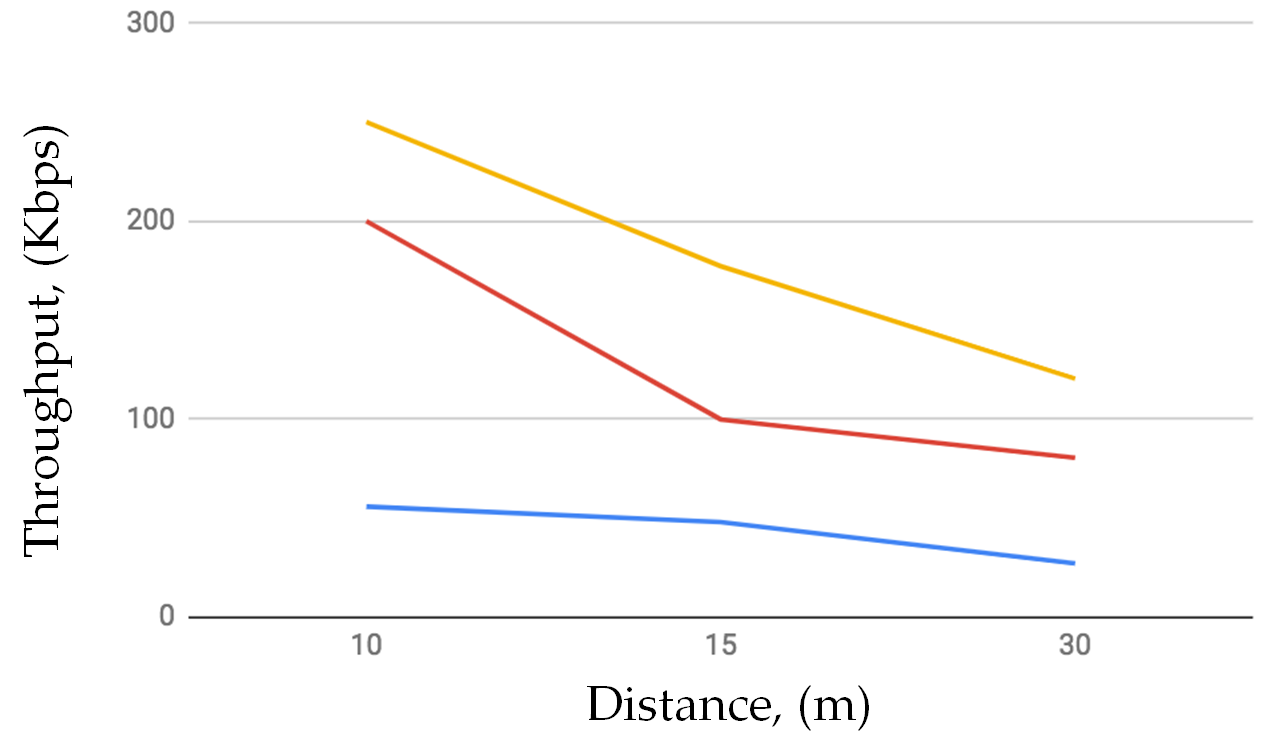
\includegraphics[width=2.9in]{BlthDist.png}
    \caption{\textit{Bluetooth Data Throughput vs Distance.} The blue line corresponds to DH1, the red line to DH3, and the yellow line to DH5. Note that the magnitude of the throughputs is significantly lower than those of WLAN.}
    \centering
    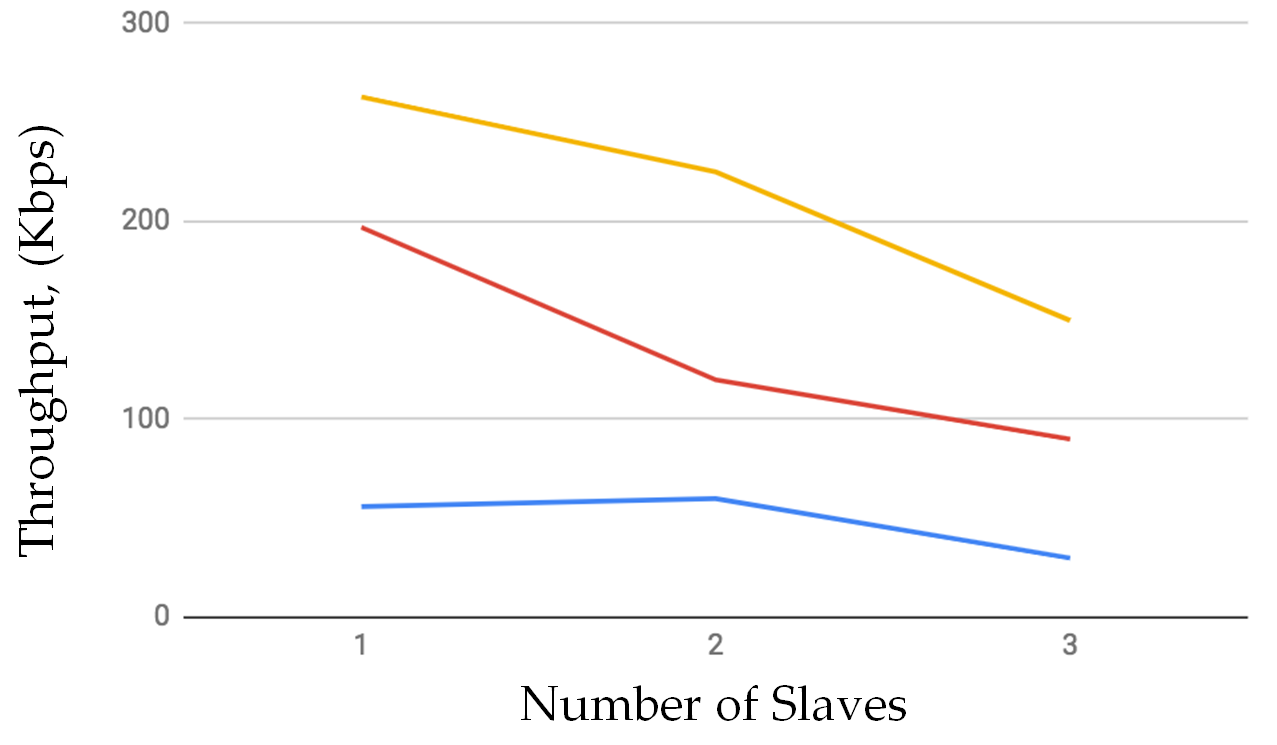
\includegraphics[width=2.9in]{BlthSlv.png}
    \caption{\textit{Bluetooth Data Throughput vs Number of Slaves in Piconet.} The blue line corresponds to DH1, the red line to DH3, and the yellow line to DH5.}
    \centering
    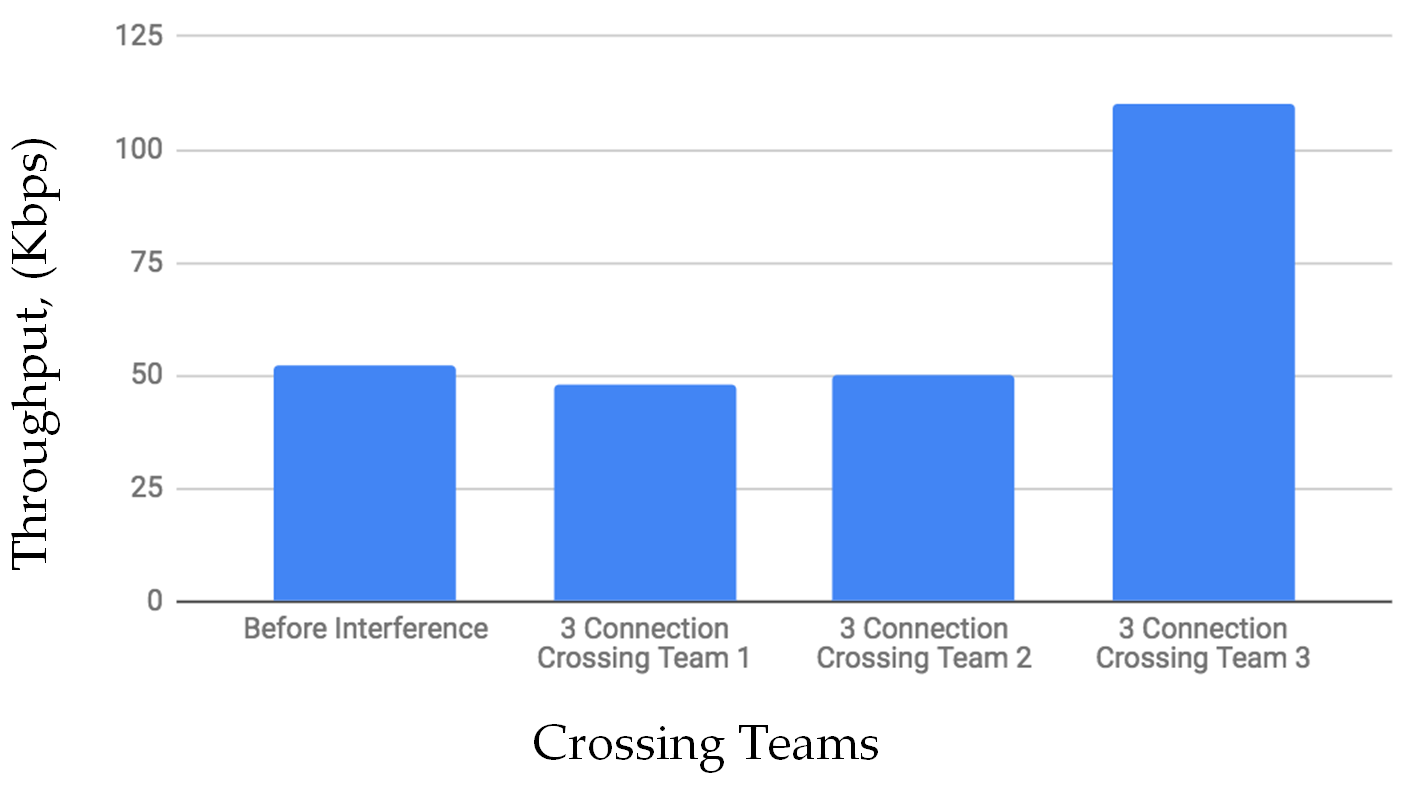
\includegraphics[width=2.9in]{Crossing.png}
    \caption{\textit{Bluetooth Data Throughput by Crossing Team.}}
\end{figure}

\begin{figure}[!htbp]
    \centering
    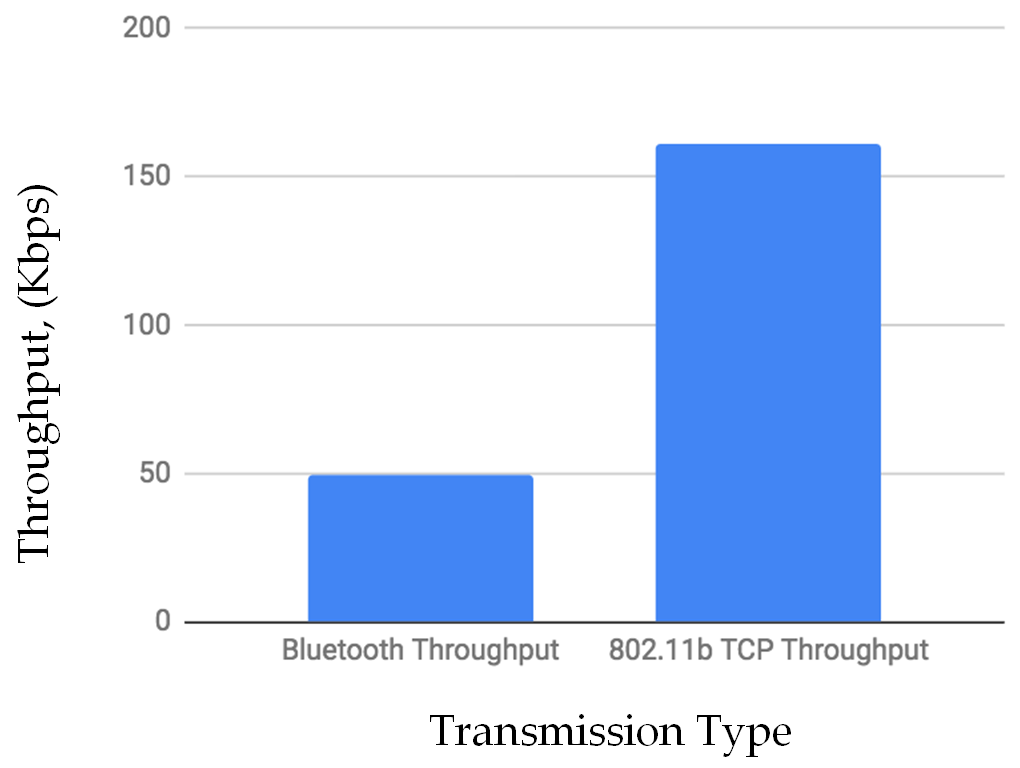
\includegraphics[width=2.9in]{Comp.png}
    \caption{\textit{Fairness of Data Throughput between Bluetooth and 802.11b.} Note the general lack of a trend.}
    \centering
\end{figure}

\hfill

\noindent Examining Figure 6, it can be seen that DH5 has a higher throughput than DH3, which in turn has a higher throughput than DH1, being the lowest. Furthermore, the difference in magnitude of throughput between Bluetooth and WLAN demonstrates the necessity of short distance communication for Bluetooth, whilst WLAN is able to support longer distance datagram transfer.

\hfill

\noindent Examining Figure 7, it can be seen that Bluetooth throughput, similar to that of WiFi, suffers as the number of slaves increase due to increased noise interference. Note the anomaly in DH1; this can be attributed to error in the experiment or the environment in which it was conducted, as the data is measured by averages which can be skewed by interference from other experiments within the room.

\hfill

\noindent The test that yielded the data for Table 8 was conducted via connecting three pairs of machines and testing interference signals from multiple piconets operating simultaneously. Examining Figure 8, it can be seen that there is no general trend among the various crossing teams.

\hfill

\noindent The test that yielded the data for Table 9 was conducted via separating two laptops by 15 feet and sending out both Bluetooth datagram packets and WiFi communication packets simultaneously. Figure 9 shows a strong trend towards the TCP throughput, implying that Bluetooth connection suffers competing with WiFi.

\newpage

%------------------------------------------------

\section{Results and Discussion}

The results of the two labs show that WiFi has significantly higher bandwidth than Bluetooth, as the TCP and UDP connections had throughputs upwards of 10 Mbps whilst Bluetooth exhibited an eighth of the throughput. It should also be noted that UDP displayed a higher average throughput than TCP, which corresponds to the lack of error recovery in UDP.

\hfill

\noindent Both distance and noise interference have notable effects on both forms of wireless communication; throughput varies inversely with distance and decreases as noise increases. It should be noted that in the experiment with the microwave that there were exceptions to this trend; however, they can be attributed to outside factors such as external noise from other teams within the same room performing other experiments.

\hfill

\noindent Lab 2 shows that the average throughput of data packet types for Bluetooth followed in order of DH5 to DH3 to DH1 from fastest to slowest. To test interference, rather than using a microwave, multiple crossings of Bluetooth devices communicating in pairs were used. Interestingly, there was no conclusive result to be drawn from this particular experiment - there was no trend. This can be attributed to factors such as noise in the surroundings along with the possibility that there is negligible difference in data throughput decrease when more Bluetooth modules are added, making Bluetooth relatively noise resilient. There was a trend, however, in that data throughput does decrease as more slaves are added to a single master node.

%------------------------------------------------

\section{Conclusions}

Bluetooth exhibits lower data rates and a steeper inverse relationship with distance than WLAN. This is reflected in usage of the two transmission types: Bluetooth is generally configured for short distance communication whilst WLAN is configured for longer distance communication. Further, it can be concluded that WLAN is the better choice for high-bandwidth transfers over long distances; UDP provides a higher throughput, but TCP is far more secure due to its handshake procedure. Bluetooth on the other hand is far better suited for short range, cheap, power-saving data transmission. It is characterized by a lower data rate but is far easier to configure, with DH5 having higher throughput than DH3 and DH1.

\hfill

\noindent The overall trends and observations adhere to the theoretical foundations covered in class. While discrepancies do exist, they are small enough to be attributed to margins of error and noise interference from various sources within Boelter itself, as the 2.4 GHz frequency is occupied by many sources.

%----------------------------------------------------------------------------------------
%	REFERENCE LIST
%----------------------------------------------------------------------------------------

\begin{thebibliography}{99} % Bibliography - this is intentionally simple in this template

\bibitem{1}
Dzhanidze, Revaz P. \textit{et al}. CS M117 Course Reader
(Univ. California Los Angeles, Los Angeles, California).

\bibitem{2}
Dzhanidze, Revaz P. \textit{et al}. CS M117 Lecure 2 W\_Channels [PPT]
(Univ. California Los Angeles, Los Angeles, California).

\bibitem{3}
Dzhanidze, Revaz P. \textit{et al}. CS M117 Lecture 3 W\_LAN 802.11 [PPT]
(Univ. California Los Angeles, Los Angeles, California).

\bibitem{4}
Dzhanidze, Revaz P. \textit{et al}. CS M117 Lecture 4 BT\_Communications [PPT]
(Univ. California Los Angeles, Los Angeles, California).

\end{thebibliography}

%----------------------------------------------------------------------------------------

\end{document}
